\begin{frame}
\frametitle{FEM error behavior}

\begin{itemize}
\item Error behavior for \hp-FEM is well understood \parencite{babuska1990}
  \begin{align*}
  \left\|\nabla\left(u \!-\! u_\text{hp}\right)\right\|_{H^{1}(\Omega)} &\leq C \, \frac{h^p}{p^{m-1}} \, \|u\|_{H^{m}(\Omega)}
  \end{align*}
\end{itemize}

\begin{itemize}
\item Exponential convergence rate possible with \hp-adaptation \parencite{babuska1996}
  \begin{align*}
  \left\|\nabla\left(u \!-\! u_\text{hp}\right)\right\|_{H^{1}(\Omega)} &\leq C \, \exp\left(- b \, N_\text{dofs}^\alpha\right)
  \end{align*}
  with $\alpha = 1/3$ in 2D and $\alpha = 1/5$ in 3D
\end{itemize}
\end{frame}





\begin{frame}
\frametitle{Kelly error estimation}

\begin{itemize}
\item Error estimator by \parencite{kelly1983}
\item Meant for generalized Poisson equation $-\nabla \cdot (a \nabla u) = f$
\item Proved to be useful in other applications as well
\end{itemize}

\begin{align*}
\|e_\text{hp}\|_{H_1(\Omega)}^2 &\leq C \sum\limits_{K \in \Omega} \eta_K^2 \\
\eta_K^2 &= \sum\limits_{F \in \partial K} c_F \int\limits_{F} \left[ a \, \frac{\partial u_\text{hp}}{\partial n} \right]^2 do \\
\left[ a \, \frac{\partial u_\text{hp}}{\partial n} \right] &= \left. a \, \frac{\partial u_\text{hp}}{\partial n_K} \right|_K + \left. a \, \frac{\partial u_\text{hp}}{\partial n_J}\right|_J
\end{align*}
\end{frame}





\begin{frame}
\frametitle{Refinement history}

\begin{minipage}{.56\textwidth}
  \begin{itemize}
    \item Verify prediction's accuracy
    \item Decide on either h- or p-adaptation on marked cells\\[.4em]
    \begin{tabular}{ll}
      Keep \textbf{\h} small: & $\eta_K > \eta_{K,\text{pred}}$ \\
      Keep \textbf{\p} large: & $\eta_K \leq \eta_{K,\text{pred}}$
    \end{tabular}
  \end{itemize}
\end{minipage}
\begin{minipage}{.43\textwidth}
  \begin{figure}
    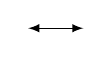
\begin{tikzpicture}[scale=0.7]
    \def\Radius{.09}
    \LagrangeCell{-4}{0}{2}{\Radius}{1}{{,,,}};
    
    \draw[>=latex, <->] (-1.5,1) -- (-.5,1);
    
    \LagrangeCell{0}{0}{1}{\Radius}{1}{{,,,}};
    \LagrangeCell{0}{1}{1}{\Radius}{1}{{,,,}};
    \LagrangeCell{1}{0}{1}{\Radius}{1}{{,,,}};
    \LagrangeCell{1}{1}{1}{\Radius}{1}{{,,,}};
    \end{tikzpicture}
    \caption{\h-adaptation}
  \end{figure}
\end{minipage}

\begin{table}
\caption{Error prediction algorithm based on \parencite{melenk2001}}
\vspace{-1em}
\begin{tabular}{ll}
  \rowcolor{fzjblue!25} \multicolumn{1}{c}{\textbf{Adaptation type}} & \multicolumn{1}{c}{\textbf{Prediction formula}} \\
  \toprule
  no adaptation & $\eta_{K,\text{pred}} = \eta_{K} \, \gamma_\text{n}$ \\
  \midrule
  \p-adaptation & $\eta_{K,\text{pred}} = \eta_{K} \,
\gamma_\text{p}^{(p_{K,\text{future}} - p_K)}$ \\
  \midrule
  \hp-refinement & $\left( \eta_{K_c,\text{pred}} \right)^2 = n_{K_c}^{-1}
\left( \eta_{K_p} \,
\gamma_\text{h} \, 0.5^{p_{K_c,\text{future}}} \,
\gamma_\text{p}^{(p_{K_c,\text{future}} - p_{K_p})} \right)^2$ \\
  \addlinespace[1mm]
  \hp-coarsening & $\left( \eta_{K_p,\text{pred}} \right)^2 = \sum\limits_{K_c} \left( \eta_{K_c} \,
(\gamma_\text{h} \, 0.5^{p_{K_p,\text{future}}})^{-1} \, \gamma_\text{p}^{(p_{K_p,\text{future}} - p_{K_c})} \right)^2$
\end{tabular}
\end{table}
\end{frame}





\begin{frame}
\frametitle{Smoothness estimation}

\begin{itemize}
\item Different representations of finite element approximation
\begin{align*}
u_{hp}(x) = \sum\limits_i u_i \, \varphi_i(x)  = \sum\limits_k c_k \, P_k(x)
\end{align*}
\end{itemize}

\begin{itemize}
\item Choose orthogonal basis $\{P_k\}$ of increasing frequency
\item Uniquely attribute frequency of oscillations to each basis function
\end{itemize}
\end{frame}





\begin{frame}
\frametitle{Orthogonal basis}

\begin{itemize}
\item Legendre: Orthogonal basis of polynomials
  \begin{align*}
  P_k(x) &= \frac{1}{2^k k!} \frac{d^k}{dx^k} \left( (x^2 - 1)^k \right) \\
  \langle P_k, P_l \rangle &= \int P_k(x) \, P_l(x) \, dx = \frac{2}{2k+1} \delta_{kl}
  \end{align*}
\end{itemize}

\begin{itemize}
\item Fourier: Orthogonal basis of sinusoids
  \begin{align*}
  P_k(x) &= \exp \left( -i \, 2 \pi k \, x \right) \\
  \langle P_k, P_l \rangle &= \int P_k(x) \, P_l^*(x) \, dx = \delta_{kl}
  \end{align*}
\end{itemize}
\end{frame}





\begin{frame}
\frametitle{Legendre polynomials}

\begin{tikzpicture}
\begin{axis}[
%cycle list/Dark2,
scale=.97,
ymin=-1.2, ymax=1.2,
xlabel=$x$,
ylabel=$P_k(x)$,
grid=major,
%legend style={at={(0.5,1.02)}, anchor=south, /tikz/every even column/.append style={column sep=0.5cm}},
%legend columns=3,
legend cell align=left,
legend pos = outer north east,
legend style={font=\tiny},
cycle list/Dark2,
every axis plot/.append style={ultra thick}
]
\addplot+[samples=2, domain=-1:1] {1};
\addlegendentry{$P_0 = 1$};

\only<2->{
\addplot+[samples=2, domain=-1:1] {x};
\addlegendentry{$P_1 = x$};
}

\only<3->{
\addplot+[samples=20, domain=-1:1] {0.5*(3*x^2-1)};
\addlegendentry{$P_2 = \frac{1}{2} \left( 3x^2 - 1 \right)$};
}

\only<4->{
\addplot+[samples=40, domain=-1:1] {0.5*(5*x^3 - 3*x)};
\addlegendentry{$P_3 = \frac{1}{2} \left( 5x^3 - 3x \right)$};
}

\only<5->{
\addplot+[samples=60, domain=-1:1] {0.125*(35*x^4 - 30*x^2 + 3)};
\addlegendentry{$P_4 = \frac{1}{8} \left( 35x^4 - 30x^2 + 3 \right)$};
}

\only<6->{
\addplot+[samples=80, domain=-1:1] {0.125*(63*x^5 - 70*x^3 + 15*x)};
\addlegendentry{$P_5 = \frac{1}{8} \left( 63x^5 - 70x^3 + 15x \right)$};
}
\end{axis}
\end{tikzpicture}
\end{frame}





\begin{frame}
\frametitle{Fourier sinusoids}

\begin{tikzpicture}
\begin{axis}[
%cycle list/Dark2,
scale=.97,
ymin=-1.2, ymax=1.2,
xlabel=$x$,
ylabel=$\operatorname{Re}\left(P_k(x)\right)$,
grid=major,
%legend style={at={(0.5,1.02)}, anchor=south, /tikz/every even column/.append style={column sep=0.5cm}},
%legend columns=3,
legend cell align=left,
legend pos = outer north east,
legend style={font=\tiny},
cycle list/Dark2,
every axis plot/.append style={ultra thick}
]
\addplot+[samples=2, domain=0:1] {1};
\addlegendentry{$P_0 = 1$};

\only<2->{
\addplot+[samples=30, domain=0:1] {cos(deg(6.28*x))};
\addlegendentry{$P_1 = \exp\left(i \, 2\pi \, x\right)$};
}

\only<3->{
\addplot+[samples=60, domain=0:1] {cos(deg(2*6.28*x))};
\addlegendentry{$P_2 = \exp\left(i \, 4\pi \, x\right)$};
}

\only<4->{
\addplot+[samples=90, domain=0:1] {cos(deg(3*6.28*x))};
\addlegendentry{$P_3 = \exp\left(i \, 6\pi \, x\right)$};
}

\only<5->{
\addplot+[samples=120, domain=0:1] {cos(deg(4*6.28*x))};
\addlegendentry{$P_4 = \exp\left(i \, 8\pi \, x\right)$};
}
\end{axis}
\end{tikzpicture}
\end{frame}





\begin{frame}
\frametitle{Decay of Legendre coefficients}

\begin{itemize}
\item Determine coefficients $\{c_k\}$ on every cell $K$:
  \begin{align*}
  c_k = \int\limits_K u_{hp}(x) \, P_k(x) \, dx
  \end{align*}
  
\item FE approximation is analytic if coefficients decay exponentially \cite{eibner2007}
  \begin{align*}
  |c_k| \leq C \exp\left( - \sigma |k| \right)
  \end{align*}
  
\item Determine decay rate $\sigma$ via least-squares fit
  \begin{align*}
  \ln(|c_k|) \sim \tilde{C} - \sigma |k|
  \end{align*}
\end{itemize}

\vspace{-1em}
\begin{block}{\vspace{-1em}}
\centering
Decay rates $\sigma$ considered as smoothness estimates \\
Keep $p$ large if $\sigma$ is large
\end{block}
\vspace{1em}
\end{frame}





\begin{frame}
\frametitle{Decay of Fourier coefficients}

\begin{itemize}
\item FE approximation is part of Hilbert space $\mathcal{H}^s$ if integral exists
  \begin{align*}
  \int\limits_K \left| \nabla^s u_{\text{hp}}(x) \right|^2 dx &= (2 \pi)^{2s} \sum\limits_k \left| c_k \right|^2 k^{2s} < \infty \\
  \Rightarrow\qquad |c_k| = \mathcal{O}&\left(k^{-\sigma - \epsilon}\right)  \quad \text{with} \quad \sigma = s + \text{dim}/2
  \end{align*}

\item Determine coefficients $\{c_k\}$ and their decay via least-squares fit on every cell $K$:
  \begin{align*}
  c_k &= \int\limits_K u_{hp}(x) \, P_k^*(x) \, dx & \ln(|c_k|) &\sim C - \sigma \ln\left( |k| \right)
  \end{align*}
\end{itemize}

\vspace{-1em}
\begin{block}{\vspace{-1em}}
\centering
Decay rates $\sigma$ considered as smoothness estimates \\
Keep $p$ large if $\sigma$ is large
\end{block}
\vspace{1em}
\end{frame}